\documentclass[conference]{IEEEtran}
\usepackage{amsmath}
\usepackage{amssymb}
\usepackage{xcolor}
\usepackage{pgfplots}
\pgfplotsset{width=7cm,compat=1.9}

\begin{document}

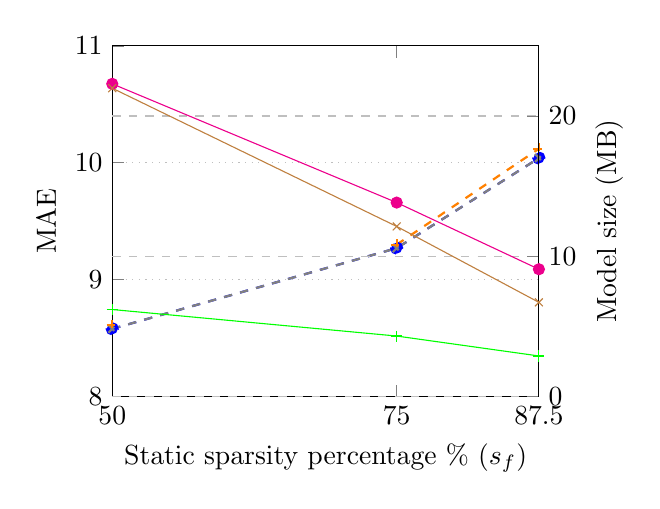
\begin{tikzpicture}

\begin{axis}[
    xlabel={Static sparsity percentage \% $(s{_f})$},
    ylabel={MAE},
    xmin=50, xmax=87.5,
    ymin=8, ymax=11,
    xtick={50,75,87.5,100},
    ymajorgrids=true,
    grid style=dotted,
    axis y line* = left, 
]

\addplot[
    dashed, 
    thick,
    color=blue,
    mark=*
 ]
    coordinates {
    (50,8.58)
(75,9.27)
(87.5,10.04)
    };
 
    
\addplot[
    dashed, 
    thick,
     color=gray,
    mark=x
 ]
    coordinates {
    (50,8.58)
(75,9.27)
(87.5,10.04)
    };
 
\addplot[
    dashed, 
    thick,
    color=orange,
     mark=+
 ]
    coordinates {
    (50,8.61)


(75,9.30)
(87.5,10.12)
    };


\end{axis}
\begin{axis}[
    ylabel={Model size (MB)},
    xmin=50, xmax=87.5,
    ymin=0, ymax=25,
    xtick={50,75,87.5,100},
    ymajorgrids=true,
    grid style=dashed,
            hide x axis,
        axis y line*=right,
]

\addplot[
    color=magenta,
    mark=*
    ]
    coordinates {
(50,22.29)
(75,13.83)
(87.5,9.08)
    };
\addplot[
    color=brown,
    mark=x
    ]
    coordinates {
(50,21.98)
(75,12.13)
(87.5, 6.72)
    };
\addplot[
    color=green,
    mark=+
    ]
    coordinates {
(50,6.21)
(75,4.32)
(87.5, 2.90)
    };

    
\end{axis}

\end{tikzpicture}

\end{document}